%template1.tex
%The following LaTeX source file represents the simplest kind of slide presentation; no overlays, no included graphics. Substitute your favorite style for ``pascal''. To create the PDF file template1.pdf, (1) be sure to use the prosper class, then (2) execute the command latex template1.tex, and (3) the command dvipdf template1.dvi.

%%%%%%%%%%%%%%%%%%%%%%%%%%%%%%% template1.tex %%%%%%%%%%%%%%%%%%%%%%%%%%%%%%%%%%%
\documentclass[a4paper,blends,pdf,colorBG,slideColor]{prosper}
% definitions for slides for CSC544
% Lutz Hamel, (c) 2007

\hypersetup{pdfpagemode=FullScreen}

\usepackage{amssymb}
\usepackage{latexsym}
\usepackage{amsmath}
%\usepackage[usenames]{color}
\usepackage{xypic}


\newcommand{\term}[1]{\ensuremath{\mbox{\bf #1}}}
\newcommand{\nonterm}[1]{\ensuremath{\mbox{#1}}}
\newcommand{\ifstmt}[3]{\ensuremath{{\bf if}\; {#1}\;{\bf then}\;{#2}\;{\bf else}\;{#3}\;\term{end}}}
\newcommand{\whilestmt}[2]{\ensuremath{{\bf while}\; {#1}\;{\bf do}\;{#2}\; \term{end}}}
\newcommand{\funcstmt}[3]{\ensuremath{{\bf fun}\; {#1}\; {\bf is}\; {#2} \; {\bf return}\; {#3}}}
\newcommand{\syntaxset}[1]{\ensuremath{\mbox{\bf #1}}}
\newcommand{\orbar}{\;|\;}
\newcommand{\bs}[1]{\begin{slide}{#1}\ptsize{8}}
\newcommand{\es}{\end{slide}}
\newcommand{\co}{\,\colon\;}
\newcommand{\pair}[2]{\ensuremath{\langle {#1}, {#2} \rangle}}
\newcommand{\encode}[1]{\ensuremath{\langle {#1} \rangle}}
\newcommand{\mytab}{\makebox[.15in]{}}
%\newcommand{\abs}[1]{{\mid{#1}\mid}}
\newcommand{\abs}[1]{{|{#1}|}}
\newcommand{\ol}[1]{\overline{#1}}

\newcommand{\qaccept}{\ensuremath{q_{\mbox{\tiny accept}}}}
\newcommand{\qreject}{\ensuremath{q_{\mbox{\tiny reject}}}}
\newcommand{\accept}{{\em accept}}
\newcommand{\reject}{{\em reject}}

\newcommand{\machine}[1]{
	\begin{quote}
	{#1}
	\end{quote}
	}

\newcommand{\fdef}[1]{
	\begin{center}
	\fbox{
	\begin{minipage}{3.5in}
	{\bf Definition:}
	{#1}
	\end{minipage}
	}
	\end{center}
	}

\newcommand{\ftheorem}[1]{
	\begin{center}
	\fbox{
	\begin{minipage}{3.5in}
	{\bf Theorem:}
	{#1}
	\end{minipage}
	}
	\end{center}
	}

\newcommand{\flemma}[1]{
	\begin{center}
	\fbox{
	\begin{minipage}{3.5in}
	{\bf Lemma:}
	{#1}
	\end{minipage}
	}
	\end{center}
	}


\newcommand{\fframe}[1]{
	\begin{center}
	\fbox{
	\begin{minipage}{3.5in}
	{#1}
	\end{minipage}
	}
	\end{center}
	}

\newcommand{\nframe}[1]{
	\begin{center}
	\begin{minipage}{3.5in}
	{#1}
	\end{minipage}
	\end{center}
	}

\begin{document}
\bs{Space Complexity}
\begin{itemize}
\item Time and space are two of the most important considerations when we seek practical solutions to computational problems.

\item Space complexity shares many of the same features of time complexity

\item Therefore, space complexity serves as a further way of classifying problems according to their computational difficulty.

\item We will continue to use the TM as our model, but now we look at the tape space it consumes during its computation.
\end{itemize}
\es


\bs{Space Complexity}
{\small
\fdef{
Let $M$ be a deterministic TM that halts on all inputs.  We define the {\bf\em space complexity} of $M$ to be the function $f\co {\mathbb N} \rightarrow {\mathbb N}$,
where $f(n)$ is the maximum number of tape cells that $M$ scans on any input of length $n$.  If the space complexity of $M$ is $f(n)$, then we also say that $M$ runs in space $f(n)$.

\vspace{.1in}

If $M$ is a nondeterministic TM wherein {\bf\em all branches halt on all inputs} we define its space complexity $f(n)$ to be the maximum number of tape cells that $M$ scans on any branch of its computation on any input of length 
$n$.
}
}
\es


\bs{Space Complexity}
{\small
\fdef{
Let $f\co {\mathbb N} \rightarrow {\mathbb R}^+$ be a function.  The {\bf\em space complexity classes}, $SPACE(f(n))$ and $NSPACE(f(n))$, are defined as follows,
\begin{eqnarray*}
SPACE(f(n)) &=& \{L | \mbox{$L$ is decided by an $O(f(n))$ space TM}\}\\
NSPACE(f(n)) &=& \{L | \mbox{$L$ is decided by an $O(f(n))$ space NTM}\}
\end{eqnarray*}
}
}
\es

\bs{$SAT \in SPACE(n)$}
{\small
\ftheorem{
\[
SAT \in SPACE(n)
\]
}
{\bf Proof:} By construction.
\begin{quote}
$M$ = "On input $\encode{\phi}$, where $\phi$ is a Boolean formula:
\begin{itemize}
\item[1.] For each truth assignment to variables $x_1,\ldots,x_m$ of $\phi$:
\item[2.]\mytab Evaluate $\phi$ on that truth assignment.
\item[3.] If $\phi$ ever evaluates to $true$, \accept; otherwise, \reject."
\end{itemize}
\end{quote}
}
This algorithm does not run in polynomial time, there are an exponential number of assignments to the variables,
\[
\underbrace{2\cdot 2\cdot\ldots\cdot 2}_m = 2^m.
\]
Therefore, as expected, this algorithms runs in $2^{O(n)}$ deterministic time where $n = \abs{\phi}$.
However, observe that it runs in $O(n)$ deterministic space.  The insight is that we can reuse the space of the variables for the various assignments but we cannot reuse the time.
\es


% for a nice proof look at Goddard's book
\bs{Savitch's Theorem}
There is an interesting relationship between deterministic and nondeterministic space complexity in the sense that simulating a nondeterministic machine on a deterministic machine incurs at most a polynomial deterministic space penalty.  Formally,
\ftheorem{{\bf (Savitch's Theorem)} For any function $f\co {\mathbb N} \rightarrow {\mathbb R}^+$, where $f(n) \ge n$,
\[
NSPACE(f(n)) \subseteq SPACE(f^2(n)).
\]
}
{\bf Proof Sketch:} Naive, brute force simulation doesn't work, but if we are clever and partition the simulation then we can reuse space -- {\em cif.} Quicksort. $\Box$\footnote{\scriptsize See website for a nice proof.  Source: Wayne Goddard, An Introduction to the Theory of Computing, 2008.}
\es

\bs{$PSPACE$}

\fdef{{\bf $PSPACE$} is the class of languages that are decidable in polynomial space on a deterministic Turing machine.  Formally,
\[
PSPACE = \bigcup_k SPACE(n^k), \mbox{ with $k > 0$}.
\]
}

Similarly, we define $NPSPACE = \bigcup_k NSPACE(n^k)$, for $k > 0$.  But from Savitch's theorem it follows that
{\small
\[
NPSPACE = PSPACE.
\]
}
\es

\bs{$NPSPACE = PSPACE$}

\ftheorem{$NPSPACE = PSPACE$}

\vspace{.2in}

{\bf Proof:} We first show that $PSPACE \subseteq NPSPACE$. For any language $L \in PSPACE$ there exists a deterministic TM that decides that language in polynomial space.  However, any deterministic TM can be seen as a special case of a non-deterministic TM.  Therefore, $L \in NPSPACE$.  It follows that $PSPACE \subseteq NPSPACE$.

We now show that the converse also holds.  Let $L \in NPSPACE$ be a language that is decided by some non-deterministic TM in polynomial space, say $L \in NSPACE(n^j)$.  Clearly, $L \in NPSPACE$.  From Savitch's Theorem we know that $NSPACE(n^j) \subseteq SPACE(n^{j+2})$.
Therefore, $L \in SPACE(n^{j+2})$.  It follows that $L \in \bigcup_k SPACE(n^k)$ and therefore $L \in PSPACE$.  This shows that
$NPSPACE \subseteq PSPACE$.

Therefore, $NPSPACE = PSPACE$.$\Box$
\es

\bs{A Hierarchy of Complexity}

We can now construct a hierarchy of complexity classes.

Observe that $P \subseteq PSPACE$.  To see this let a machine execute in $t(n) \ge n$ polynomial time.  But this implies that the machine can use at most $t(n)$ polynomial space (one cell per computation step).

In a similar argument we have $NP \subseteq NPSPACE$ and from the argument above $NP \subseteq PSPACE$.

We already know that $P \subseteq NP$.

Finally, if we have a $f(n) \ge n$ polynomial space machine it can be shown that this machine runs in
at most $2^{O(f(n))}$ exponential time.  Thus, $PSPACE \subseteq EXPTIME$.

\[
P \subseteq NP \subseteq PSPACE \subseteq EXPTIME.\footnote{It is believed that all the set containments are proper.}
\]

\vspace{.2in}
\es


\bs{A Hierarchy of Complexity}
\begin{center}
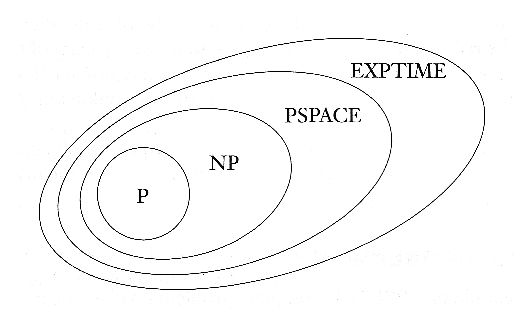
\includegraphics[height=60mm]{images/complexity-hierarchy.eps}
\end{center}
\es

\end{document}
%%%%%%%%%%%%%%%%%%%%%%%%%%% end of template1.tex %%%%%%%%%%%%%%%%%%%%%%%%%%%%%%%%

